Last time, we introduced the path integral in quantum mechanics, and we said it took the form
\begin{equation}
    \bra{x}e^{-iHt/\hbar}\ket{x_0}=\int \cD x e^{iS[x]/\hbar}.
\end{equation}
Let us consider now a ``rotation'' to imaginary time, $t\to - i\tau$ (Wick rotation). Then our path integral becomes
\begin{equation}
    \bra{x}e^{-H\tau/\hbar}\ket{x_0}=\int \cD x e^{-S[x]/\hbar}.
\end{equation}
Working with a real exponent has some benefits-- the convergence of the integral is more obvious, and in the $\hbar \to 0$ limit we expect the integral to be dominated by the classical path $x$ which minimizes the action $S[x].$

We can now observe that 1D quantum mechanics is like a $0+1$D quantum field theory-- the field is simply
\begin{equation*}
    x(t): \RR \to \RR.
\end{equation*}
In fact, 3D quantum mechanics is also like a $0+1$D QFT, where the field is now
\begin{equation*}
    \vec x(t): \RR \to \RR^3.
\end{equation*}
Given a single spacetime label $t$, a QM theory gives us a real scalar in $\RR$ or a vector in $\RR^3$-- cf. Srednicki Ch. 1. There are different approaches to quantization, but in the \term{second quantization} formalism we demote position $\vec x$ from an operator $\hat x$ to a label on a spacetime point $(\vec x,t)$. Therefore QFT in $3+1$ dimensions has e.g. a scalar field $\phi$ which is a map
\begin{equation*}
    \phi: \RR^{1,3}\to \RR.
\end{equation*}

\subsection*{Path integral methods}
Let's begin with the simplest possible case, QFT in zero dimensions.%
    \footnote{Cf. Skinner Ch. 2, Srednicki \textsection 8,9.}
All of spacetime is a single point $p$,%
    \footnote{If you're reading my SUSY notes, you should be getting d\'ej\`a vu right about now.}
and our (real scalar) field $\phi$ is a map $\phi:\set{p}\to\RR$.

Using our imaginary time (Euclidean signature) convention for the path integral, we write
\begin{equation}
    Z = \int_\RR d\phi\, e^{-S[\phi]/\hbar}.
\end{equation}
We'll take our action $S[\phi]$ to be polynomial in $\phi$, with highest power even.

As in statistical field theory, we are interested in correlation functions and expectation values. Given a function $f(\phi)$, we might like to compute the expectation value
\begin{equation}
    \avg{f}=\frac{1}{Z} \int d\phi \, f(\phi)e^{-S[\phi]/\hbar}.
\end{equation}
For this to have a chance of convergence, $f$ should not grow too rapidly as $|\phi| \to \infty$. Usually the functions we are interested in are polynomial in $\phi$.

\subsection*{Free field theory}
Suppose we have $N$ real scalar fields $\phi_a, a=1,\ldots, N$. We can compactly write this as a single field
\begin{equation}
    \phi: \set{p}\to \RR^N,
\end{equation}
and we'd like to compute the integral
\begin{equation}
    Z_0 = \int d^N\, \phi e^{-S[\phi]/\hbar}.
\end{equation}
Now, a free theory simply means that the action is quadratic in our fields. A priori it could have included kinetic terms, but since we are in zero dimensions, there are no derivatives to take and therefore no kinetic terms in this model. Then we can write our action as
\begin{equation}
    S(\phi)=\frac{1}{2} \cM_{ab} \phi_a \phi_b =\frac{1}{2} \phi^T \cM \phi,
\end{equation}
where $\cM$ is an $N\times N$ symmetric matrix with $\det M > 0$. So our action could include terms like $\frac{1}{2}\phi_1^2$ and $\frac{5}{2} \phi_1 \phi_4$. Since $\cM$ is symmetric, we can diagonalize it as
\begin{equation*}
    \cM=P\Lambda P^T
\end{equation*}
for some orthogonal matrix $P$. But equivalently we could just redefine our fields to some new fields $\phi'= P^T  \phi$ so that 
\begin{equation*}
    S(\phi)= \frac{1}{2} \phi'{}^T \Lambda \phi'= \frac{1}{2} \sum_{i=1}^N \lambda_i (\phi'_i)^2,
\end{equation*}
where $\lambda_i$ are the eigenvalues of $\cM$. Since $P$ is orthogonal, $\det P = 1 \implies d^N \phi=(\det P)d^N \phi' = d^N \phi'$, so our path integral separates into $N$ Gaussian integrals of the form
\begin{equation}
    \int_{-\infty}^\infty dx\, e^{-\frac{\lambda}{2\hbar}x^2}=\sqrt{\frac{2\pi \hbar}{\lambda}}.
\end{equation}
Thus
\begin{equation}
    Z_0 = \int d^N \phi \, e^{-\frac{1}{2\hbar}\phi^T \cM \phi}= \prod_{i=1}^N d \phi_i \, e^{-\frac{1}{2\hbar} \lambda_i (\phi_i)^2} = \frac{(2\pi \hbar)^{N/2}}{\sqrt{\det \cM}}.
\end{equation}

We can now  introduce a source term $J$, modifying our action to
\begin{equation}
    S(\phi)=\frac{1}{2} \phi^T \cM \phi + J\cdot \phi.
\end{equation}
If we complete the square and make a change of variables $\tilde \phi= \phi+ \cM^{-1} J,$
we find that the new path integral with a source is
\begin{align*}
    Z_0[J] &= \int d^N \phi \, \exp \bkt{-\frac{1}{2\hbar} \phi^T \cM \phi -\frac{1}{\hbar} J \cdot \phi}\\
        &= \exp\paren{\frac{1}{2\hbar}J^T \cM^{-1} J} \int d^N \tilde \phi\, e^{-\frac{1}{2\hbar} \tilde \phi^T \cM \tilde \phi}\\
        &= Z_0 \exp\paren{\frac{1}{2\hbar} J^T \cM^{-1} J}.
\end{align*}
We see that $\P{}{J}$ derivatives will bring down $\phi$s, which will allow us to compute correlation functions just like we did in statistical physics with the partition function.

\begin{exm}
    What is the value of the correlation function $\avg{\phi_a \phi_b}$ in this theory? We can compute it directly:
    \begin{align*}
        \avg{\phi_a \phi_b} &= \frac{1}{Z_0}\left.\int d^N \phi \, \phi_a \phi_b \exp\bkt{-\frac{1}{2\hbar} \phi^T \cM \phi -\frac{1}{\hbar} J \cdot \phi}\right|_{J=0}\\
            &= \frac{1}{Z_0} \int d^N \phi \paren{-\hbar \P{}{J_a}} \paren{-\hbar \P{}{J_b}} \left.\exp \bkt{-\frac{1}{2\hbar} \phi^T \cM \phi -\frac{1}{\hbar} J \cdot \phi}\right|_{J=0}\\
            &= (-\hbar)^2 \P{}{J_a}\P{}{J_b} \left.\exp\bkt{\frac{1}{2\hbar} J^T \cM^{-1} J}\right|_{J=0}\\
            &= \hbar (\cM^{-1})_{ab}.
    \end{align*}
    Note that the first $J$ derivative brings down an $\cM^{-1}J$ (so our expression is of the form $\cM^{-1} J \exp (J^T \cM^{-1} J)$), and when we take the second $J$ derivative, we will get two terms, one of the form $\cM^{-1}\exp(\ldots)$ and another of the form $(\cM^{-1}J)^2 \exp(\ldots)$. The second term is zero when we set $J=0$, and the exponential becomes $1$ in both cases, so we are just left with $\cM^{-1}$. 
\end{exm}
What we have calculated is a two-point function, otherwise known as a propagator (though it's a bit silly to call this a propagator when the spacetime is just a single point). We can associate a Feynman diagram to this process:
%
\begin{center}
    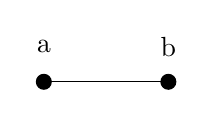
\begin{tikzpicture}[x=0.75pt,y=0.75pt,yscale=-1,xscale=1]
        
        %Straight Lines [id:da8887105125657073] 
        \draw    (200,123) -- (260,123) ;
        \draw  [color={black}  ][fill={black}  ][line width=0.75]      (200, 123) circle [x radius= 3.35, y radius= 3.35]   ;
        \draw  [color={black}  ][fill={black}  ][line width=0.75]      (260, 123) circle [x radius= 3.35, y radius= 3.35]   ;
        
        % Text Node
        \draw (200,106) node  [align=left] {a};
        % Text Node
        \draw (260,106) node  [align=left] {b};
    
    \end{tikzpicture}
\end{center}

There is another method we can use to compute propagators (cf. Osborn \textsection 1.3):
\begin{align*}
    \cM_{ca} \avg{\phi_a \phi_b} &= \frac{1}{Z_0} 
        \int d^N \phi \,\cM_{ca} \phi_a \phi_b \exp\bkt{-\frac{1}{2\hbar} \phi^T \cM \phi}\\
        &= -\frac{\hbar}{Z_0} \int d^N \phi \, \phi_b \P{}{\phi_c} \exp\bkt{-\frac{1}{2\hbar} \phi^T \cM \phi}\\
        &= \frac{\hbar}{Z_0}\int d^N \phi\, \P{\phi_b}{\phi_c} \exp\bkt{-\frac{1}{2\hbar} \phi^T \cM \phi}\\
        &= \hbar \delta_{bc} \implies \avg{\phi_a \phi_b}=\hbar (\cM^{-1})_{ab}.
\end{align*}
In going from the second to the third line, we have integrated by parts to move the $\P{}{\phi_c}$ to $\phi_b,$ and then recognized the remaining integral as $Z_0$.

More generally, let $l(\phi)= l \cdot \phi = \sum_{a=1}^N l_a \phi_a (\neq 0)$ be a linear function of $\phi$, with $l_a \in \RR.$ Then the expected value $\avg{l_a(\phi) \ldots l_p(\phi)}$ is given by
\begin{equation*}
    \avg{l_a(\phi) \ldots l_p(\phi)} = 
        (-\hbar)^p \prod_{i=1}^p \paren{l_i \P{}{J_i}} \left.\frac{Z_0[J]}{Z_0}\right|_{J=0}.
\end{equation*}

Notice that if we play this game for an odd number of $J_i$ derivatives, all our terms will be of the form $J^p \exp(\ldots)$ where $p$ is odd. When we set $J=0$, all these terms therefore vanish, which tells us that $\avg{\phi_{a_1}\ldots \phi_{a_p}}=0$ for $n$ odd. If we compute it for $p=2k, k\in \NN$, the terms that survive setting $J=0$ will have $k$ factors of $\cM^{-1}$.

\begin{exm}
    What is the value of the four-point function $\avg{\phi_a \phi_b \phi_c \phi_d}$ in free field theory? It is simply
    \begin{equation*}
        \avg{\phi_a \phi_b \phi_c \phi_d} =\hbar^2 \bkt{(\cM^{-1})_{ab} (\cM^{-1})_{cd} + (\cM^{-1})_{ac} (\cM^{-1})_{bd} + (\cM^{-1})_{ad} (\cM^{-1})_{bc}}.
    \end{equation*}
    Though we haven't said it, this is effectively a toy version of Wick's theorem-- we are taking contractions of the fields using $(\cM^{-1})$s as propagators.
    
    We can depict these contractions as connecting some $2k$ dots pairwise with lines using a simplified Feynman diagram notation:
    
    \begin{center}
    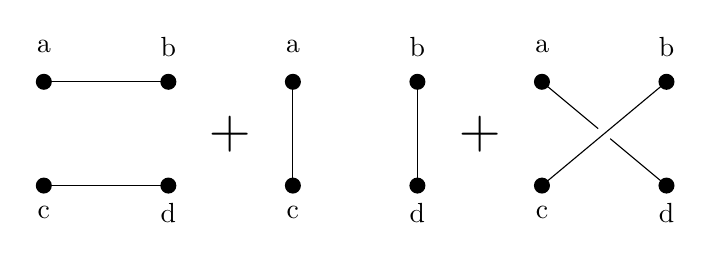
\begin{tikzpicture}[x=0.75pt,y=0.75pt,yscale=-1,xscale=1]
    %uncomment if require: \path (0,300); %set diagram left start at 0, and has height of 300
        
        %Straight Lines [id:da8887105125657073] 
        \draw    (100,123) -- (160,123) ;
        \draw [shift={(100,123)}, rotate = 0] [color={black}  ][fill={black}  ][line width=0.75]      (0, 0) circle [x radius= 3.35, y radius= 3.35]   ;
        \draw [shift={(160,123)}, rotate = 0] [color={black}  ][fill={black}  ][line width=0.75]      (0, 0) circle [x radius= 3.35, y radius= 3.35]   ;
        
        % Text Node
        \draw (100,106) node  [align=left] {a};
        % Text Node
        \draw (160,106) node  [align=left] {b};
        
        %Straight Lines [id:da8887105125657073] 
        \draw    (100,173) -- (160,173) ;
        \draw [shift={(100,173)}, rotate = 0] [color={black}  ][fill={black}  ][line width=0.75]      (0, 0) circle [x radius= 3.35, y radius= 3.35]   ;
        \draw [shift={(160,173)}, rotate = 0] [color={black}  ][fill={black}  ][line width=0.75]      (0, 0) circle [x radius= 3.35, y radius= 3.35]   ;
        
        % Text Node
        \draw (100,186) node  [align=left] {c};
        % Text Node
        \draw (160,186) node  [align=left] {d};
        %%end first diagram
        \draw (190,148) node  [align=center] {\huge$+$};
        
        %Straight Lines [id:da8887105125657073] 
        \draw    (220,123) -- (220,173) ;
        \draw [shift={(220,123)}, rotate = 0] [color={black}  ][fill={black}  ][line width=0.75]      (0, 0) circle [x radius= 3.35, y radius= 3.35]   ;
        \draw [shift={(280,123)}, rotate = 0] [color={black}  ][fill={black}  ][line width=0.75]      (0, 0) circle [x radius= 3.35, y radius= 3.35]   ;
        
        % Text Node
        \draw (220,106) node  [align=left] {a};
        % Text Node
        \draw (280,106) node  [align=left] {b};
        
        %Straight Lines [id:da8887105125657073] 
        \draw    (280,123) -- (280,173) ;
        \draw [shift={(220,173)}, rotate = 0] [color={black}  ][fill={black}  ][line width=0.75]      (0, 0) circle [x radius= 3.35, y radius= 3.35]   ;
        \draw [shift={(280,173)}, rotate = 0] [color={black}  ][fill={black}  ][line width=0.75]      (0, 0) circle [x radius= 3.35, y radius= 3.35]   ;
        
        % Text Node
        \draw (220,186) node  [align=left] {c};
        % Text Node
        \draw (280,186) node  [align=left] {d};
        %%end second diagram
        \draw (310,148) node  [align=center] {\huge$+$};
        
        %Straight Lines [id:da8887105125657073] 
        \draw    (340,123) -- (400,173) ;
        \draw [shift={(340,123)}, rotate = 0] [color=black  ][fill={black}  ][line width=0.75]      (0, 0) circle [x radius= 3.35, y radius= 3.35]   ;
        \draw [shift={(400,123)}, rotate = 0] [color={black}  ][fill={black}  ][line width=0.75]      (0, 0) circle [x radius= 3.35, y radius= 3.35]   ;
        
        % Text Node
        \draw (340,106) node  [align=left] {a};
        % Text Node
        \draw (400,106) node  [align=left] {b};
        
        %make the lines look like they cross over
        \draw [shift={(370, 148)}] [color={white}] [fill={white}] (0, 0) circle [x radius= 3.5, y radius= 3.5] ;
        
        %Straight Lines [id:da8887105125657073] 
        \draw    (340,173) -- (400,123) ;
        \draw [shift={(340,173)}, rotate = 0] [color={black}  ][fill={black}  ][line width=0.75]      (0, 0) circle [x radius= 3.35, y radius= 3.35]   ;
        \draw [shift={(400,173)}, rotate = 0] [color={black}  ][fill={black}  ][line width=0.75]      (0, 0) circle [x radius= 3.35, y radius= 3.35]   ;
        
        % Text Node
        \draw (340,186) node  [align=left] {c};
        % Text Node
        \draw (400,186) node  [align=left] {d};
    \end{tikzpicture}
\end{center}
    
    In general, the number of distinct ways we can pair $2k$ elements is
    \begin{equation*}
        \frac{(2k)!}{2^k  k!}.
    \end{equation*}
    The logic here is that we could take all $(2k)!$ permutations of the $2k$ elements, and then take neighboring pairs, e.g. if our elements are $\set{a,b,c,d,e,f}$, one set of pairs is
    \begin{equation*}
        abdcfe\to ab|dc|fe.
    \end{equation*}
    The order of the $2$ elements in each of the $k$ pairs doesn't matter ($ab|dc=ba|dc$), so we've overcounted by a factor of $2^k$, and the order of all the $k$ pairs also doesn't matter ($ab|dc=dc|ab$), so we divide by another factor of $k!$ to get the final result.
\end{exm}

\begin{exm}
    One last example-- if our free fields are instead complex, $\phi:\set{p}\to \CC$, then $\cM$ is hermitian. Therefore $(\cM^{-1})$ will in general not be symmetric, and so the order of the indices matters. That is, $\avg{\phi_a \phi_b^*}=\hbar (\cM^{-1})_{ab}$. Then the associated Feynman diagram has an arrow to indicate direction:
    
    \begin{center}
        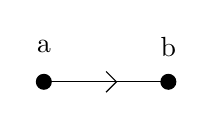
\begin{tikzpicture}[x=0.75pt,y=0.75pt,yscale=-1,xscale=1]
            
            %Straight Lines [id:da8887105125657073] 
            \draw    (200,123) -- (260,123) ;
            \draw    (230,118) -- (235,123) -- (230,128);
            \draw  [color={black}  ][fill={black}  ][line width=0.75] (200, 123) circle [x radius= 3.35, y radius= 3.35]   ;
            \draw [color={black}] [fill={black}][line width=0.75]      (260, 123) circle [x radius= 3.35, y radius= 3.35]   ;
            
            % Text Node
            \draw (200,106) node  [align=left] {a};
            % Text Node
            \draw (260,106) node  [align=left] {b};
        
        \end{tikzpicture}
    \end{center}
\end{exm}

